\chapter{Experimente și analiza rezultatelor}

\section{Setul de date}

În cadrul acestui proiect, pentru evaluarea performanței modelului propus, a fost utilizat setul de date \textbf{CK+ (Cohn-Kanade Extended Dataset)}, unul dintre cele mai utilizate seturi de date publice pentru recunoașterea expresiilor faciale în mediul controlat.

\subsection*{Descrierea datelor}
Setul de date CK+ conține înregistrări faciale reale, fiind compus din secvențe video ce surprind trecerea de la o expresie neutră la vârful (apexul) unei emoții specifice. 
Link-ul oficial pentru accesarea setului de date este: \url{http://www.pitt.edu/~emotion/ck-spread.htm}.

Caracteristicile principale ale subsetului utilizat sunt:
\begin{itemize}
	\item \textbf{Categorii:} Există 7 clase de emoții etichetate: 1. Furie (Anger), 2. Dispreț (Contempt), 3. Dezgust (Disgust), 4. Frică (Fear), 5. Fericire (Happiness), 6. Tristețe (Sadness), 7. Surpriză (Surprise).
	\item \textbf{Structura secvențelor:} Pentru fiecare subiect și fiecare ipostază, au fost extrase câte 10 cadre (frames), care acoperă evoluția temporală a expresiei.
	\item \textbf{Dimensiune imagini:} Imaginile au fost redimensionate la o rezoluție de $48 \times 48$ pixeli pentru a optimiza procesul de calcul.
\end{itemize}

\subsection*{Distribuția datelor pe fold-uri}
Pentru a asigura o evaluare robustă, s-a utilizat o strategie de \textbf{10-fold cross-validation}, folosind seed-ul 42 pentru reproductibilitate. Distribuția celor 309 secvențe pe cele 10 fold-uri este prezentată în Tabelul \ref{tab:distributie_date}.

\begin{table}[h!]
	\centering
	\caption{Distribuția emoțiilor pe cele 10 fold-uri (CK+)}
	\label{tab:distributie_date}
	\begin{tabular}{@{}ccccccccc@{}}
		\toprule
		\textbf{Fold} & \textbf{Anger} & \textbf{Contempt} & \textbf{Disgust} & \textbf{Fear} & \textbf{Happiness} & \textbf{Sadness} & \textbf{Surprise} & \textbf{Total} \\ \midrule
		1 & 5 & 2 & 6 & 3 & 7 & 3 & 8 & 34 \\
		2 & 5 & 2 & 6 & 3 & 7 & 3 & 8 & 34 \\
		3 & 5 & 1 & 6 & 3 & 7 & 3 & 8 & 33 \\
		4 & 5 & 1 & 6 & 3 & 7 & 3 & 8 & 33 \\
		5 & 5 & 1 & 5 & 2 & 7 & 3 & 8 & 31 \\
		6 & 4 & 1 & 5 & 2 & 7 & 3 & 8 & 30 \\
		7 & 4 & 1 & 5 & 2 & 7 & 3 & 8 & 30 \\
		8 & 4 & 1 & 5 & 2 & 7 & 3 & 7 & 29 \\
		9 & 4 & 1 & 5 & 2 & 7 & 2 & 7 & 28 \\
		10 & 4 & 1 & 5 & 2 & 6 & 2 & 7 & 27 \\ \midrule
		\textbf{Total} & \textbf{45} & \textbf{12} & \textbf{54} & \textbf{24} & \textbf{69} & \textbf{28} & \textbf{77} & \textbf{309} \\ \bottomrule
	\end{tabular}
\end{table}

\section{Metodologie de antrenare și evaluare}

\subsection*{Arhitectura modelului și paradigma de învățare}
Modelul implementat se bazează pe o rețea neuronală cu impulsuri (\textit{Spiking Neural Network} - SNN) cu o arhitectură convoluțională 3D, capabilă să proceseze atât informația spațială, cât și pe cea temporală din secvențele video.

Paradigma de învățare utilizată este una de tip \textbf{STDP (Spike-Timing-Dependent Plasticity)}, specific regula \textit{Biological STDP}. Aceasta permite ajustarea greutăților sinaptice în funcție de corelația temporală a impulsurilor dintre neuronii pre-sinaptici și post-sinaptici.

\subsection*{Preprocesarea datelor}
Înainte de a fi introduse în rețea, datele trec prin următoarele etape:
\begin{enumerate}
	\item \textbf{Filtrare On/Off:} Utilizarea unui \texttt{DefaultOnOffFilter} pentru evidențierea contrastelor și a marginilor (mărime filtru 7, parametri 0.1 și 1.0).
	\item \textbf{MaxScaling:} Normalizarea intensității pixelilor.
	\item \textbf{Latency Coding:} Conversia pixelilor în impulsuri (spikes), unde intensitatea este codificată prin latența temporală a primului impuls.
\end{enumerate}

\subsection*{Configurarea stratului convoluțional și hiper-parametri}
Nucleul modelului este reprezentat de un strat de convoluție 3D (\texttt{Convolution3D}). Parametrii utilizați pentru antrenare sunt detaliați în Tabelul \ref{tab:hiperparametri}.

\begin{table}[h!]
	\centering
	\caption{Hiper-parametrii rețelei SNN}
	\label{tab:hiperparametri}
	\begin{tabular}{ll}
		\toprule
		\textbf{Parametru} & \textbf{Valoare} \\ \midrule
		Număr de filtre & 64 \\
		Dimensiune filtru (WxHxD) & $5 \times 5 \times 3$ \\
		Număr de epoci & 800 \\
		Threshold inițial ($\theta$) & 4.0 \\
		$t_{obj}$ (Time Objective) & 0.80 \\
		Learning rate Threshold ($\mu_{th}$) & 0.09 \\
		Learning rate Greutăți ($\mu_{w}$) & 0.009 \\
		Spatial Pooling (output size) & $4 \times 4$ \\
		Temporal Pooling (output size) & 2 \\
		\bottomrule
	\end{tabular}
\end{table}

\subsection*{Evaluarea și Clasificarea}
După extragerea trăsăturilor prin stratul convoluțional SNN și aplicarea metodelor de \textit{SumPooling} și \textit{TemporalPooling}, reprezentările finale sunt clasificate folosind un algoritm \textbf{SVM (Support Vector Machine)}. Evaluarea se face prin cross-validation pe cele 10 fold-uri menționate anterior.

\section{Metrici de evaluare}

\begin{itemize}\item \textbf{Metrici Globale de Clasificare:}\begin{itemize}\item \textbf{Acuratețea (Accuracy):} Proporția predicțiilor corecte din totalul eșantioanelor:
		
		\[ \text{Accuracy} = \frac{N_{correct}}{N_{total}} \times 100\% \]
		
		\textbf{Matricea de Confuzie:} Reprezentare tabelară pentru identificarea erorilor sistematice între emoții similare (ex. \textit{fear} vs \textit{surprise}).\end{itemize}
	
	\item \textbf{Metrici Specifice Straturilor SNN (Per Layer Analysis):}
	\begin{itemize}
		\item \textbf{Activitatea Neuronală (Activity):} Reprezintă rata de declanșare a spike-urilor în cadrul stratului. 
		\begin{itemize}
			\item \textit{Importanță:} Un neuron care emite un spike tinde să își reducă la tăcere vecinii (inhibiție laterală). Analiza activității este esențială pentru menținerea stării de \textbf{homeostazie} a rețelei.
		\end{itemize}
		\item \textbf{Coerența (Coherence):} Măsoară gradul de redundanță al trăsăturilor învățate. 
		\begin{itemize}
			\item \textit{Interpretare:} O coerență scăzută indică faptul că SNN-ul a învățat o varietate mare de trăsături distincte. Antrenamentul eficient trebuie să tindă spre o anumită \textbf{incoerență} pentru a maximiza capacitatea de reprezentare.
		\end{itemize}
	\end{itemize}
\end{itemize}

\subsubsection{Activitatea Neuronală (Activity)}
Reprezintă dinamica de descărcare a spike-urilor în raport cu topologia stratului.

\begin{itemize}
	\item \textbf{Sparsity (Raritatea):} Se calculează pe baza raportului dintre norma $L_1$ și norma $L_2$ a activărilor. 
	\begin{itemize}
		\item \textit{Interval optim:} O valoare cuprinsă între \textbf{0.7 și 0.9} este ideală. O raritate prea mare (spre 1.0) indică o rețea "moartă", în timp ce o valoare mică indică o activitate densă, care anulează avantajul energetic al SNN.
	\end{itemize}
	\item \textbf{Active Units (\%):} Procentul de neuroni care emit cel puțin un spike per eșantion.
	\begin{itemize}
		\item \textit{Interval optim:} Pentru straturi convoluționale, o activitate de \textbf{1\% - 5\%} este considerată biologic plauzibilă și eficientă computațional.
	\end{itemize}
	\item \textbf{Quiet (\%):} Procentul de eșantioane pentru care stratul nu a generat niciun spike.
	\begin{itemize}
		\item \textit{Interpretare:} Această valoare trebuie să fie cât mai aproape de \textbf{0\%}. O valoare ridicată (ex. >10\%) sugerează că pragul de activare (\textit{threshold}) este prea înalt sau că datele de intrare nu sunt normalizate corect.
	\end{itemize}
\end{itemize}

\subsubsection{Coerența Trăsăturilor (Coherence)}
Măsoară similitudinea spectrală între nucleele (kernel-urile) de convoluție prin calcularea similitudinii cosinus între vectorii de ponderi $w_i$ și $w_j$.

\begin{equation}
	\text{Coherence}(w_i, w_j) = \frac{w_i \cdot w_j}{\|w_i\| \|w_j\| + \epsilon}
\end{equation}

\begin{itemize}
	\item \textbf{Interpretarea Cuartilelor (Q1, Q2, Q3):}
	\begin{itemize}
		\item \textit{Interval optim (Mediana/Q2):} O valoare sub \textbf{0.3 - 0.5} indică o rețea sănătoasă care a învățat trăsături diverse (margini, texturi diferite). 
		\item \textit{Riscuri:} Dacă \textit{Max} și \textit{Q3} tind spre \textbf{0.9 - 1.0}, rețeaua suferă de redundanță extremă (mai mulți neuroni au învățat exact aceeași trăsătură), ceea ce limitează capacitatea de discriminare a emoțiilor.
	\end{itemize}
	\item \textbf{Importanța Incoerenței:} Un grad ridicat de decorelare între filtre este esențial pentru ca algoritmul de clasificare ulterior (SVM sau FC) să poată extrage informație utilă din spațiul trăsăturilor.
\end{itemize}


\section{Rezultate obținute și analiză}

În această secțiune sunt prezentate performanțele obținute în urma procesului de cross-validation, precum și o analiză detaliată a comportamentului rețelei la nivel de distribuție a datelor și a impulsurilor (\textit{spikes}).

\subsection*{Performanța pe fold-uri}

Rezultatele clasificării pentru fiecare dintre cele 10 fold-uri sunt centralizate în Tabelul \ref{tab:rezultate_folds}. Rata medie de clasificare obținută este de aproximativ \textbf{48.02\%}.

\begin{table}[h!]
	\centering
	\caption{Acuratețea clasificării pe fiecare fold}
	\label{tab:rezultate_folds}
	\begin{tabular}{@{}ccc@{}}
		\toprule
		\textbf{Fold} & \textbf{Rata de clasificare (\%)} & \textbf{Corecte / Total} \\ \midrule
		Fold 1 & 58.82\% & 20/34 \\
		Fold 2 & 47.05\% & 16/34 \\
		Fold 3 & 51.51\% & 17/33 \\
		Fold 4 & 45.45\% & 15/33 \\
		Fold 5 & 41.93\% & 13/31 \\
		Fold 6 & 53.33\% & 16/30 \\
		Fold 7 & 50.00\% & 15/30 \\
		Fold 8 & 48.27\% & 14/29 \\
		Fold 9 & 35.71\% & 10/28 \\
		Fold 10 & 48.14\% & 13/27 \\ \midrule
		\textbf{Medie} & \textbf{48.02\%} & \textbf{159 / 309} \\ \bottomrule
	\end{tabular}
\end{table}

\subsection*{Analiza detaliată pe Fold 1}
Fold-ul 1 a înregistrat cea mai ridicată performanță (58.82\%). Pentru a înțelege punctele forte și limitările modelului, matricea de confuzie pentru Fold 1 (Tabelul \ref{tab:confusion_matrix}), surprinde corelarea etichetelor reale (\textit{True Label}) cu probabilitățile maxime generate de clasificatorul SVM.

\begin{table}[h!]
	\centering
	\caption{Matricea de confuzie pentru Fold 1 (34 secvențe)}
	\label{tab:confusion_matrix}
	\begin{tabular}{r|ccccccc|c}
		\toprule
		\textbf{Real \textbackslash Prezis} & \textbf{1} & \textbf{2} & \textbf{3} & \textbf{4} & \textbf{5} & \textbf{6} & \textbf{7} & \textbf{Recall \%} \\ \midrule
		\textbf{1 (Anger)}     & 0 & 0 & 5 & 0 & 0 & 0 & 0 & 0.0\% \\
		\textbf{2 (Contempt)}  & 1 & 0 & 1 & 0 & 0 & 0 & 0 & 0.0\% \\
		\textbf{3 (Disgust)}   & 0 & 0 & \textbf{6} & 0 & 0 & 0 & 0 & 100.0\% \\
		\textbf{4 (Fear)}      & 0 & 0 & 0 & 0 & 0 & 0 & 3 & 0.0\% \\
		\textbf{5 (Happiness)} & 0 & 0 & 0 & 0 & \textbf{7} & 0 & 0 & 100.0\% \\
		\textbf{6 (Sadness)}   & 1 & 0 & 2 & 0 & 0 & 0 & 0 & 0.0\% \\
		\textbf{7 (Surprise)}  & 0 & 0 & 1 & 0 & 0 & 0 & \textbf{7} & 87.5\% \\ \midrule
		\textbf{Precision \%}  & 0.0\% & 0.0\% & 40.0\% & 0.0\% & 100.0\% & 0.0\% & 70.0\% & \textbf{Acc: 58.8\%} \\
		\bottomrule
	\end{tabular}
\end{table}

\subsubsection{Interpretarea erorilor de clasificare}
Analiza probabilităților individuale relevă câteva fenomene tipice pentru procesarea imaginilor faciale prin SNN:

\begin{itemize}
	\item \textbf{Suprapunerea caracteristicilor Furie-Dezgust:} Toate secvențele de \textit{Anger} (clasa 1) au primit probabilitatea maximă pentru \textit{Disgust} (clasa 3). Acest lucru se explică prin similitudinea morfologică a acestor expresii (încrețirea nasului și coborârea sprâncenelor), pe care filtrele convoluționale actuale le extrag ca fiind identice.
	\item \textbf{Dificultatea detectării Fricii:} Emoția \textit{Fear} (clasa 4) a fost clasificată sistematic drept \textit{Surprise} (clasa 7). Din punct de vedere vizual, ambele emoții implică deschiderea largă a ochilor și ridicarea sprâncenelor. Rezultatele sugerează că modelul reușește să detecteze activarea musculară, dar nu și subtilitatea temporală care diferențiază frica de surpriză.
	\item \textbf{Performanță Robustă la Emoții Extreme:} Clasele \textit{Happiness} și \textit{Disgust} au un \textit{recall} de 100\%, indicând faptul că arhitectura SNN propusă este extrem de eficientă în izolarea trăsăturilor de intensitate mare (zâmbet larg, respectiv contracție nazală pronunțată).
	\item \textbf{Clasele sub-reprezentate:} \textit{Contempt} și \textit{Sadness} au înregistrat performanțe slabe, fiind confundate cu emoții negative mai „puternice”. Aceasta este o limitare cunoscută a setului de date CK+, unde aceste clase au mult mai puține exemple de antrenament.
\end{itemize}

\subsection*{Analiza distribuției valorilor și a impulsurilor}
Pentru a înțelege modul în care stratul convoluțional procesează informația, am extras distribuția globală a valorilor înainte și după aplicarea stratului de convoluție 3D.

\subsubsection{Distribuția după Latency Encoding (Input)}
În faza de preprocesare, valorile sunt codificate temporal. Distribuția prezentată în Tabelul \ref{tab:dist_input} arată o concentrație masivă a valorilor în intervalul $[0.9 - 1.0]$ (peste 72\%), ceea ce indică faptul că majoritatea neuronilor de intrare generează impulsuri cu latență mare.

\subsubsection{Distribuția după Stratul Convoluțional (Spikes)}
După trecerea prin stratul de convoluție, se observă o menținere a densității în zona superioară, dar cu o ușoară redistribuire. Această activitate intensă în intervalul $[0.8 - 1.0]$ sugerează că filtrele convoluționale au identificat numeroase corelații spațio-temporale în secvențele video de intrare.

\begin{table}[h!]
	\centering
	\caption{Analiza comparativă a distribuției valorilor (Fold 1)}
	\label{tab:dist_input}
	\begin{tabular}{@{}ccc@{}}
		\toprule
		\textbf{Interval} & \textbf{Înainte de Conv (Input) \%} & \textbf{După Conv (Spikes) \%} \\ \midrule
		$[0.0 - 0.5]$ & 1.66\% & 0.01\% \\
		$[0.5 - 0.6]$ & 1.71\% & 0.14\% \\
		$[0.6 - 0.7]$ & 3.37\% & 1.24\% \\
		$[0.7 - 0.8]$ & 6.57\% & 6.34\% \\
		$[0.8 - 0.9]$ & 14.01\% & 22.49\% \\
		$[0.9 - 1.0]$ & 72.68\% & 69.78\% \\ \bottomrule
	\end{tabular}
\end{table}

\subsection*{Interpretarea rezultatelor}
Analiza distribuției arată că rețeaua nu suferă de \textit{vanishing spikes}, având o activitate susținută. Totuși, rata de clasificare medie sugerează că, deși anumite emoții cu trăsături faciale distincte (precum fericirea sau surpriza) sunt ușor de separat, distincția între emoțiile subtile (furie vs. dezgust) necesită o rafinare a hiper-parametrilor sau o creștere a numărului de filtre pentru a surprinde diferențe mai fine de textură și mișcare.
Deși rata medie de 48.02\% indică un potențial ridicat pentru recunoașterea emoțiilor de intensitate mare (Happiness, Disgust), se observă o dificultate în discriminarea stărilor afective subtile. Această limitare este pusă pe seama numărului redus de eșantioane pentru clase precum Contempt, dar și pe natura nesupervizată a algoritmului STDP, care prioritizează frecvența trăsăturilor în detrimentul discriminabilității lor. Optimizarea viitoare a pragului de activare ($\theta$) și a ratei de învățare a pragului ($\mu_{th}$) ar putea conduce la o mai bună specializare a filtrelor.

\subsection*{Vizualizarea și analiza hărților de trăsături (Feature Maps)}

Pentru a investiga modul în care modelul \textit{Convolutional SNN} extrage informația din secvențele video, au fost vizualizate hărțile de trăsături (\textit{feature maps}) generate de stratul convoluțional. Această analiză este esențială pentru a valida capacitatea regulii de învățare STDP de a codifica tipare spațio-temporale relevante fără supraveghere.

\subsubsection{Impactul mecanismului TimeObjectiveOutput}

O componentă critică în arhitectura propusă este etapa de conversie a output-ului. În Figura \ref{fig:anger_before_after} este ilustrat efectul aplicării transformării \texttt{OutputConverter.TimeObjectiveOutput} asupra unei secvențe de \textit{Anger}.

\begin{figure}[h!]
	\centering
	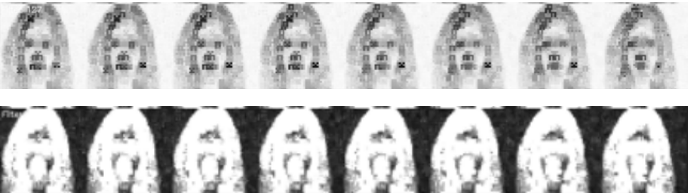
\includegraphics[width=0.9\textwidth]{figures/models/feature_maps_csnn/selection/anger-before-after.png}
	\caption{Vizualizarea hărților de trăsături pentru clasa Anger: Sus - activări brute (pre-procesare); Jos - activări după aplicarea TimeObjectiveOutput.}
	\label{fig:anger_before_after}
\end{figure}

Analiza vizuală relevă următoarele aspecte:
\begin{itemize}
	\item \textbf{Normalizarea Latenței:} În varianta brută, activările sunt difuze, având un raport semnal-zgomot scăzut. Aplicarea \texttt{TimeObjectiveOutput} forțează latențele spre valoarea țintă $t_{obj}=0.8$, rezultând într-o reprezentare mult mai clară a contururilor faciale.
	\item \textbf{Evidențierea Dinamicii:} După procesare, se observă o focalizare a impulsurilor în zonele cu mișcare musculară intensă (frunte, ochi, gură). Această „curățare” a semnalului permite clasificatorului SVM să lucreze cu trăsături mai bine definite, minimizând redundanța spațială.
\end{itemize}

\subsection*{Analiza calitativă a hărților de trăsături per emoție}

În Figurile \ref{fig:fmaps_1} și \ref{fig:fmaps_2} sunt prezentate seturile de hărți de trăsături extrase pentru cele 7 categorii de emoții. Fiecare eșantion este reprezentat printr-o succesiune de cadre ce reflectă intensitatea activării neuronale. În paradigma \textit{Latency Coding}, zonele albe (pixeli cu intensitate mare) corespund unor latențe mici, indicând o declanșare rapidă a impulsurilor ca răspuns la trăsături faciale proeminente.

\begin{figure}[h!]
	\centering
	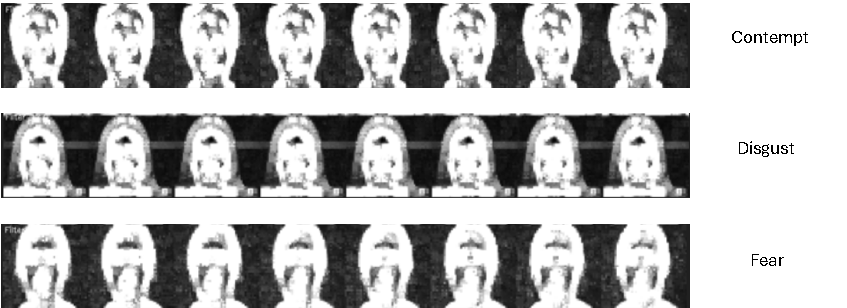
\includegraphics[width=0.85\textwidth]{figures/models/feature_maps_csnn/selection/feature-maps-1.png}
	\caption{Hărți de trăsături pentru clasele Contempt, Disgust și Fear.}
	\label{fig:fmaps_1}
\end{figure}

\begin{figure}[h!]
	\centering
	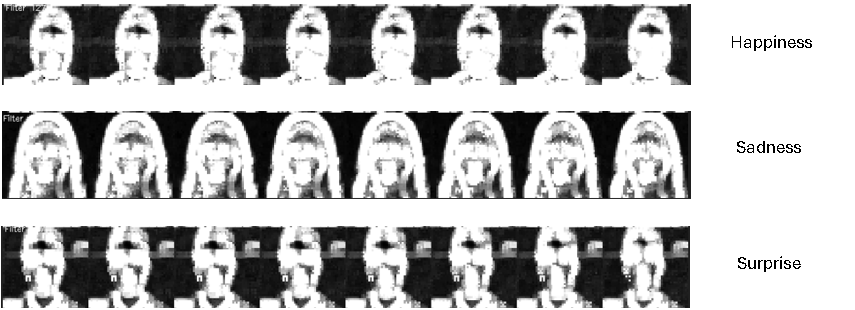
\includegraphics[width=0.85\textwidth]{figures/models/feature_maps_csnn/selection/feature-maps-2.png}
	\caption{Hărți de trăsături pentru clasele Happiness, Sadness și Surprise.}
	\label{fig:fmaps_2}
\end{figure}

\subsubsection{Corelația dintre trăsături și performanța clasificării}

Observarea hărților de trăsături permite explicarea rezultatelor obținute în matricea de confuzie:

\begin{itemize}
	\item \textbf{Happiness și Disgust:} Aceste clase prezintă zone de activare extrem de bine localizate (comisurile bucale pentru fericire și zona nazală pentru dezgust). Caracterul distinctiv al acestor impulsuri timpurii explică rata de \textit{recall} de 100\% pentru aceste clase.
	\item \textbf{Surprise vs. Fear:} Hărțile de trăsături confirmă similitudinea vizuală între cele două emoții. În ambele cazuri, filtrele SNN detectează deschiderea largă a ochilor, însă distribuția spațială a impulsurilor este aproape identică, ceea ce conduce la clasificarea sistematică a fricii drept surpriză.
	\item \textbf{Sadness și Contempt:} Aceste emoții generează hărți cu o densitate mai mică a impulsurilor („pete” mai întunecate), indicând o mișcare facială de intensitate redusă. Această activitate rarefiată face ca trăsăturile extrase să fie mai puțin robuste în fața zgomotului, explicând performanța scăzută pe aceste clase.
\end{itemize}

Această analiză vizuală demonstrează că modelul SNN propus a învățat să acționeze ca un extractor de trăsături fiziologice, reușind să mapeze corelările spațio-temporale din clipurile video în latențe neuronale discriminative.

\subsubsection{Vizualizarea nucleelor convoluționale (Greutăți Sinaptice)}

Pentru o înțelegere aprofundată a modului în care s-a realizat adaptarea sinaptică prin procesul STDP nesupervizat, au fost extrase greutățile sinaptice ale celor 64 de filtre după cele 800 de epoci de antrenament pe Fold 1. Vizualizarea acestor nuclee (\textit{kernels}) de dimensiune $5 \times 5 \times 3$ este prezentată în Figura \ref{fig:kernels_fold_1}. Deoarece un nucleu este tridimensional (spatial $5 \times 5$ pe o adâncime temporală $3$), vizualizarea este o proiecție color a volumului de greutăți.

\begin{figure}[h!]
	\centering
	% Asigură-te că imaginea ta este redenumită sau salvată sub acest nume în folderul proiectului
	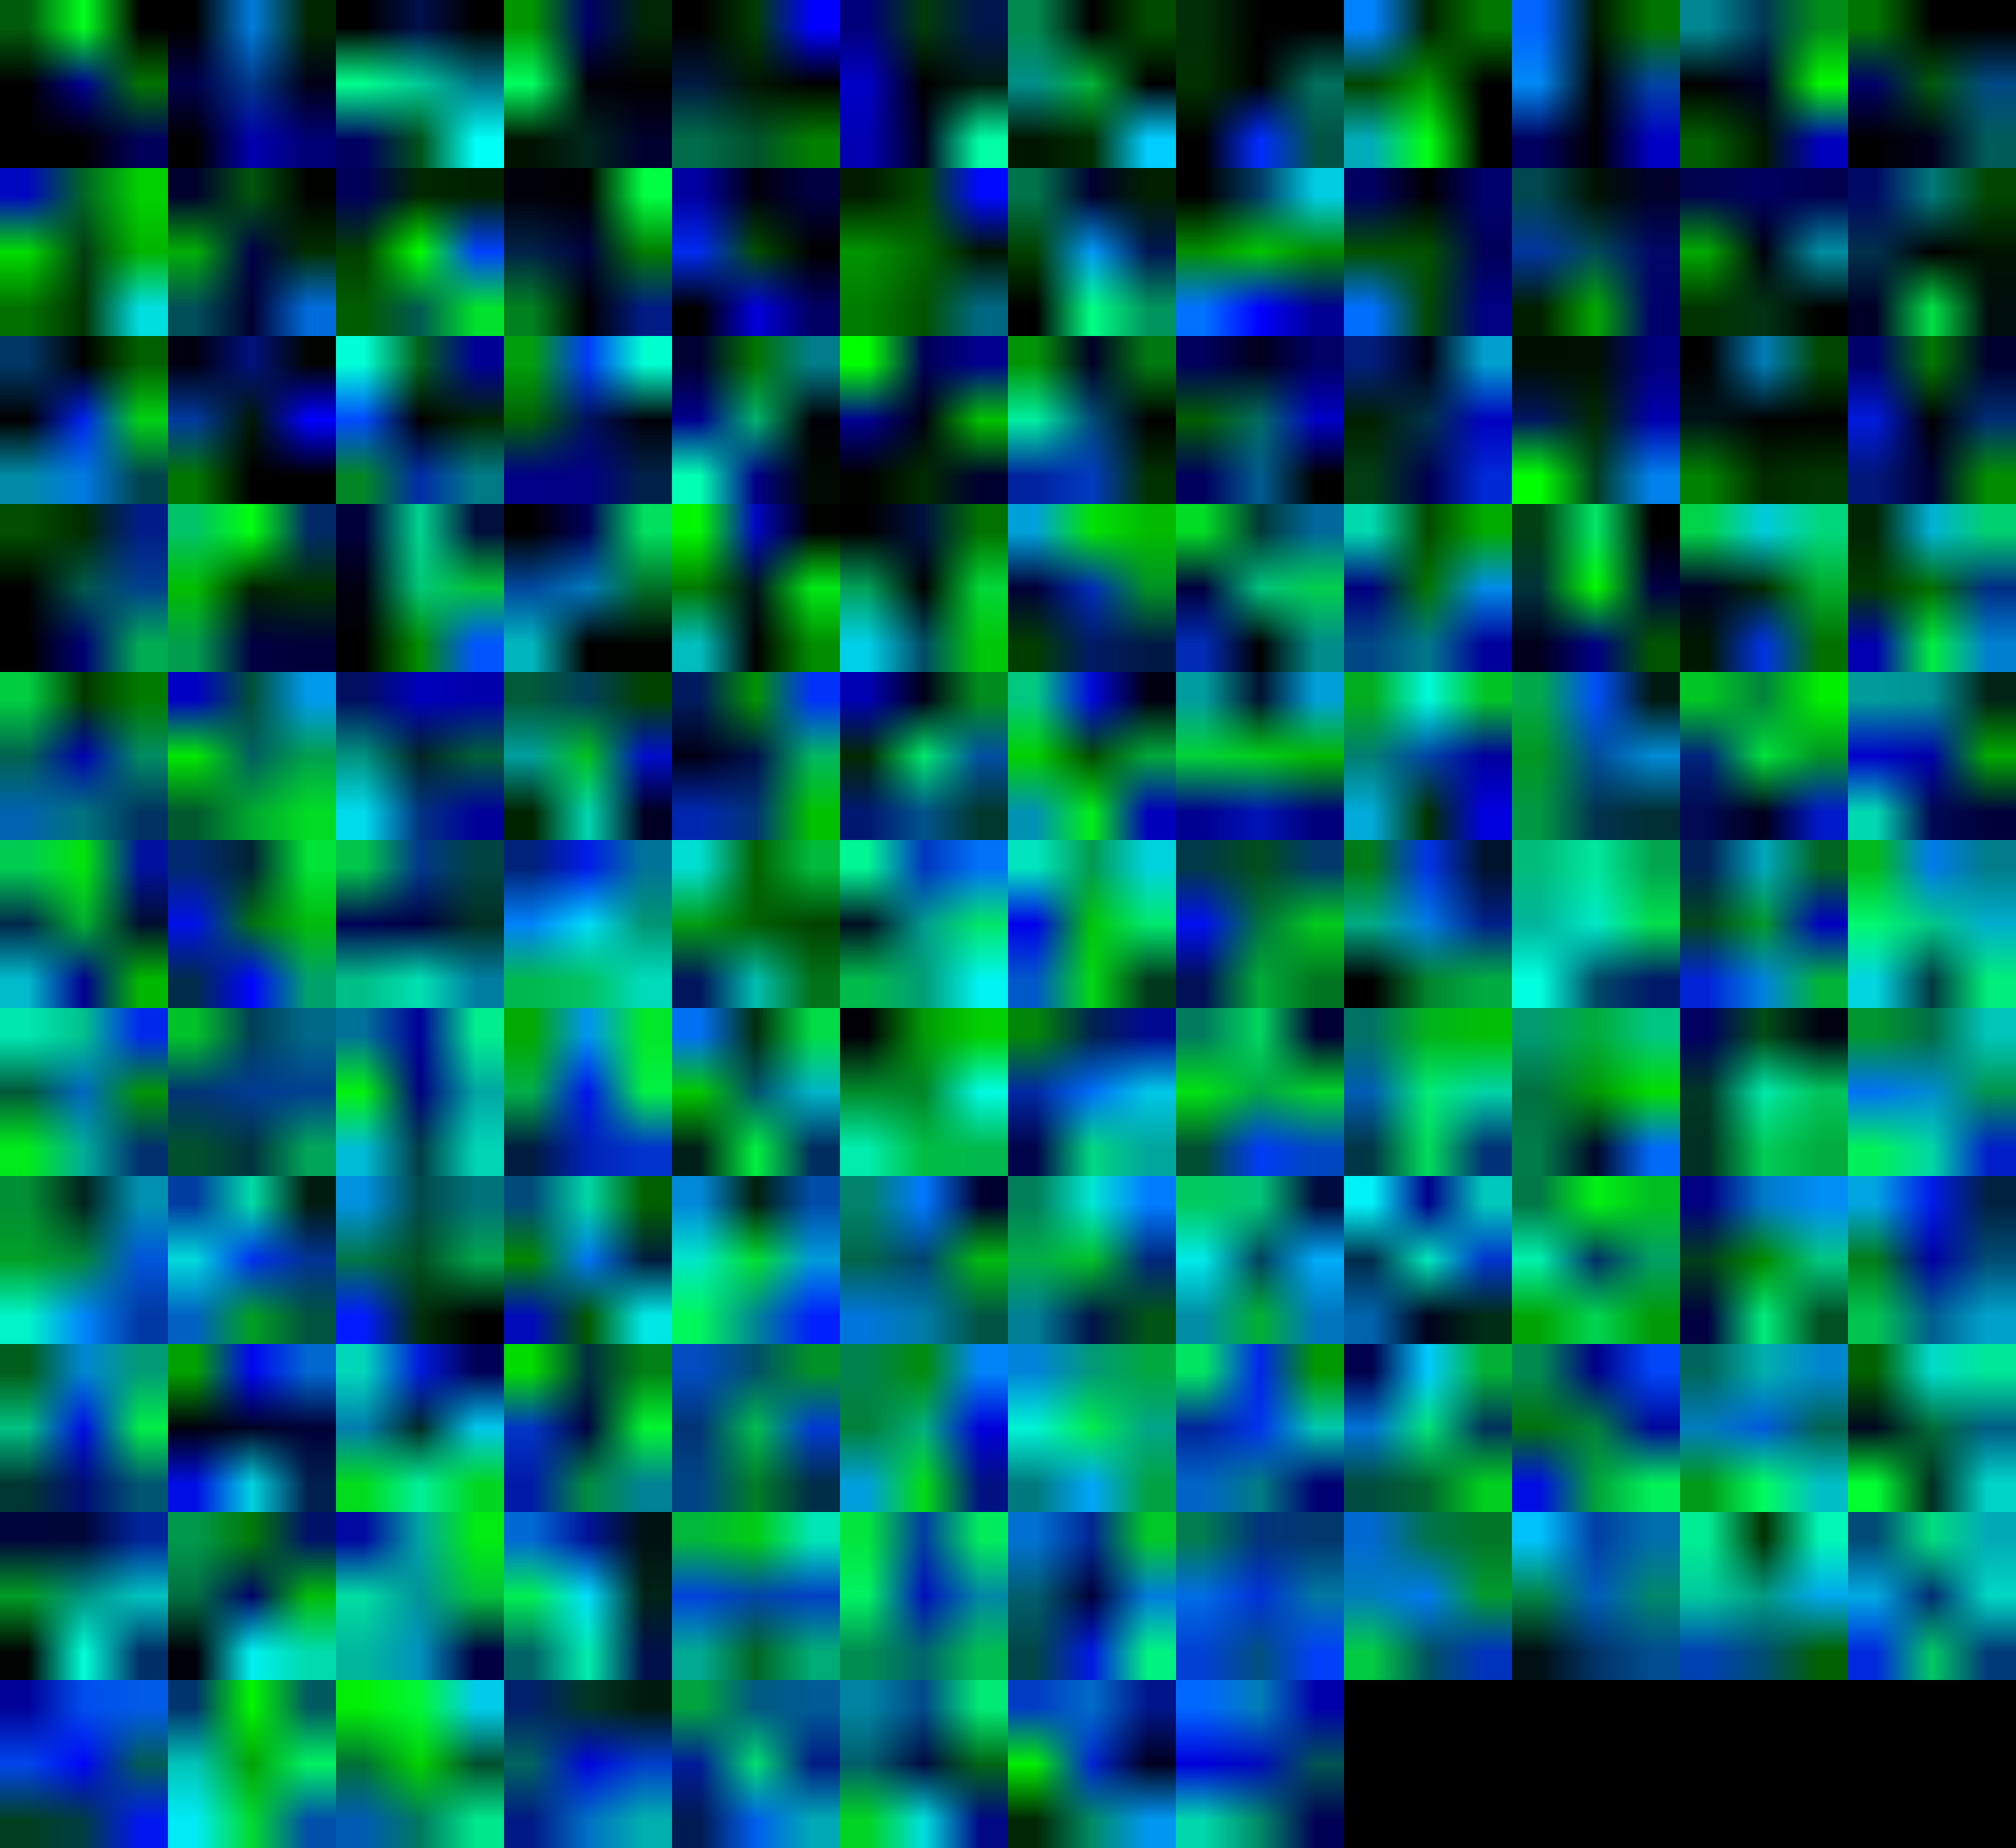
\includegraphics[width=0.6\textwidth]{figures/models/kernels_csnn/kernels_fold_1.png} 
	\caption{Vizualizarea celor 64 de nuclee convoluționale ($8 \times 8$ filtre) învățate de SNN pe Fold 1. Culoarea reprezintă magnitudinea și polaritatea greutăților sinaptice (nivele de potențiere și depresie).}
	\label{fig:kernels_fold_1}
\end{figure}

Analiza calitativă a Figura \ref{fig:kernels_fold_1} relevă tipare caracteristice învățării STDP nesupervizate pe secvențe video:

\begin{itemize}
	\item \textbf{High-Frequency Spatial Variance:} Nucleele prezintă o variație spațială ridicată, aspectul lor fiind aparent zgomotos. Acest fenomen este caracteristic etapelor inițiale de specializare a filtrelor în SNN-uri nesupervizate. În loc să învețe margini orientate generice (cum ar fi filtrele Gabor), STDP-ul tinde să specializeze nucleele pe tipare foarte locale și specifice de corelații temporale de impulsuri, prezente în datele de intrare.
	\item \textbf{Validarea Incoerenței:} Aspectul divers și aparent aleatoriu al filtrelor este, paradoxal, un rezultat dorit. Așa cum s-a menționat în secțiunea \ref{sec:metrici} (definiția coerenței), antrenamentul eficient trebuie să tindă spre o incoerență ridicată. Faptul că filtrele nu sunt identice și nu prezintă trăsături repetitive validează succesul regulii de învățare STDP în a evita redundanța și în a acoperi un spectru larg de variații ale datelor.
	\item \textbf{Limitările învățării trăsăturilor globale:} Absența unor structuri globale clar definite în kernels explică performanța scăzută pe clasele subtile. Filtrele sunt suficient de discriminate pentru a distinge între schimbări majore de intensitate (zâmbet vs. contracție nazală), dar nu au învățat încă să reprezinte deformări fine ale feței pe care clasificatorul liniar ulterior (SVM) să le poată separa eficient.
\end{itemize}

\section{Analiză Comparativă și Validarea Modelului}

Pentru a evalua relevanța trăsăturilor extrase de stratul convoluțional SNN, a fost realizat un experiment de control (baseline). În cadrul acestuia, clasificatorul SVM a fost antrenat direct pe pixelii imaginilor brute (\textit{raw pixels}), eliminând complet componenta de spiking și procesarea STDP.

\subsection*{Configurația modelului de referință (Baseline)}
Modelul de referință utilizează un strat de tip \texttt{layer::Stream}, care acționează ca o funcție identitate, pasând datele de intrare direct către etapele de pooling, fără nicio preprocesare sau filtrare temporală. Configurația utilizată este următoarea:

\begin{itemize}
	\item \textbf{Input:} Pixeli raw (fără \textit{Latency Coding}).
	\item \textbf{Pooling:} \texttt{SumPooling} ($4 \times 4$) și \texttt{TemporalPooling} (2), identic cu modelul SNN pentru a asigura o comparație echitabilă a spațiului de trăsături.
	\item \textbf{Clasificator:} SVM liniar.
\end{itemize}

\subsection*{Rezultate comparative}

Rezultatele obținute prin cross-validation pentru ambele abordări sunt centralizate în Tabelul \ref{tab:comparatie_rezultate}.

\begin{table}[h!]
	\centering
	\caption{Comparație între SVM pe pixeli raw și arhitectura propusă (SNN + SVM)}
	\label{tab:comparatie_rezultate}
	\begin{tabular}{@{}ccc@{}}
		\toprule
		\textbf{Fold} & \textbf{SVM Pixeli Raw (\%)} & \textbf{SNN + SVM (Propus) (\%)} \\ \midrule
		Fold 1 & 44.11\% & 58.82\% \\
		Fold 2 & 38.23\% & 47.05\% \\
		Fold 3 & 54.54\% & 51.51\% \\
		Fold 4 & 39.39\% & 45.45\% \\
		Fold 5 & 38.70\% & 41.93\% \\
		Fold 6 & 36.66\% & 53.33\% \\
		Fold 7 & 43.33\% & 50.00\% \\
		Fold 8 & 44.82\% & 48.27\% \\
		Fold 9 & 39.28\% & 35.71\% \\
		Fold 10 & 37.03\% & 48.14\% \\ \midrule
		\textbf{Medie} & \textbf{41.61\%} & \textbf{48.02\%} \\ \bottomrule
	\end{tabular}
\end{table}

\subsection*{Interpretarea superiorității modelului SNN}

Compararea performanțelor evidențiază un câștig net de \textbf{6.41\%} în favoarea arhitecturii bazate pe SNN. Această diferență, deși aparent modestă în cifre absolute, este semnificativă din punct de vedere al procesării bio-inspirate:

\begin{enumerate}
	\item \textbf{Extracția de trăsături (Feature Extraction):} Diferența de performanță confirmă faptul că nucleele învățate prin STDP nu sunt aleatorii; ele reușesc să distileze informația vizuală în „puncte de interes” temporale care sunt mai ușor de separat liniar de către un SVM decât pixelii bruti.
	\item \textbf{Reducerea zgomotului:} În timp ce pixelii raw conțin multă informație redundantă (fundal, variații de iluminare), SNN-ul, prin filtrarea On/Off și Latency Coding, se concentrează pe marginile dinamice (schimbările de expresie), oferind un input mai „curat” pentru clasificator.
	\item \textbf{Analiza cazurilor particulare:} Se observă că în aproape toate fold-urile (cu excepția fold-ului 3 și 9), SNN-ul depășește baseline-ul. În Fold 1, saltul este de la 44.11\% la 58.82\% (+14.71\%), ceea ce indică faptul că pentru anumite secvențe video, reprezentarea prin impulsuri este net superioară celei spațiale clasice.
\end{enumerate}

În concluzie, rezultatele demonstrează validitatea ipotezei de lucru: rețelele neuronale cu impulsuri, antrenate nesupervizat, sunt capabile să extragă trăsături temporale relevante pentru recunoașterea expresiilor faciale, îmbunătățind capacitatea de generalizare a sistemului față de procesarea directă a imaginilor.

\section{Modelul de Înaltă Performanță: Arhitectura Hibridă CNN-LSTM}

Pentru a oferi un termen de comparație raportat la standardele actuale de \textit{Deep Learning} și pentru a echipa aplicația finală cu un motor de predicție robust, a fost implementată o arhitectură hibridă de tip \textbf{CNN-LSTM}. Acest model combină puterea de extracție a trăsăturilor spațiale ale unei rețele convoluționale pre-antrenate cu capacitatea rețelelor recurente de a modela evoluția temporală a emoțiilor.

\subsection*{Descrierea Arhitecturii}

Modelul propus utilizează un mecanism de \textit{Feature Extraction} urmat de un modul de memorie temporală:
\begin{enumerate}
	\item \textbf{Extractorul Spațial (Backbone):} S-a utilizat modelul \textbf{ResNet18}, pre-antrenat pe setul de date ImageNet. S-a păstrat structura până la stratul de \textit{Adaptive Average Pooling}, rezultând un vector de trăsături de dimensiune 512 pentru fiecare cadru video.
	\item \textbf{Modulul Temporal (LSTM):} Trăsăturile extrase sunt introduse într-un strat \textbf{LSTM} (\textit{Long Short-Term Memory}) cu o dimensiune ascunsă de 256. Acesta analizează succesiunea celor 10 cadre pentru a identifica „apexul” emoției.
	\item \textbf{Capul de Clasificare:} Un modul de tip \textit{Fully Connected} cu \textit{Dropout} (0.5) și activare ReLU realizează maparea finală către cele 7 clase de emoții.
\end{enumerate}

\subsection*{Strategia de Antrenament în Două Faze}

Pentru a maximiza performanța pe un set de date de dimensiuni medii precum CK+, s-a adoptat o strategie de \textit{Transfer Learning} structurată în două etape:
\begin{itemize}
	\item \textbf{Faza 1 (Warm-up):} Înghețarea parametrilor CNN și antrenarea exclusivă a modulelor LSTM și FC timp de 10 epoci (LR=$10^{-3}$). Acest lucru permite modelului temporal să se adapteze la trăsăturile extrase de ResNet.
	\item \textbf{Faza 2 (Fine-tuning):} Dezghețarea selectivă a ultimului bloc convoluțional (\textit{Layer 4}) din ResNet și antrenarea întregului ansamblu timp de 30 de epoci cu un \textit{Learning Rate} scăzut ($10^{-4}$) și \textit{Cosine Annealing}.
\end{itemize}

\subsection*{Rezultate Obținute}

Performanța modelului CNN-LSTM, evaluată prin 10-fold cross-validation, este prezentată în Tabelul \ref{tab:rezultate_cnn_lstm}.

\begin{table}[h!]
	\centering
	\caption{Acuratețea modelului CNN-LSTM pe cele 10 fold-uri}
	\label{tab:rezultate_cnn_lstm}
	\begin{tabular}{@{}lc|lc@{}}
		\toprule
		\textbf{Fold} & \textbf{Acuratețe (\%)} & \textbf{Fold} & \textbf{Acuratețe (\%)} \\ \midrule
		Fold 1 & 87.88\% & Fold 6 & 85.71\% \\
		Fold 2 & 85.71\% & Fold 7 & 93.75\% \\
		Fold 3 & 81.82\% & Fold 8 & 89.66\% \\
		Fold 4 & 87.50\% & Fold 9 & 78.57\% \\
		Fold 5 & 96.97\% & Fold 10 & 96.15\% \\ \midrule
		\textbf{Medie} & \multicolumn{3}{c}{\textbf{88.37\% $\pm$ 5.65\%}} \\ \bottomrule
	\end{tabular}
\end{table}

\section{Sinteza Rezultatelor și Concluzii Experimentale}

În Tabelul \ref{tab:sinteza_finala} este prezentată comparația finală între cele trei abordări investigate în cadrul acestei lucrări.

\begin{table}[h!]
	\centering
	\caption{Comparație centralizată a modelelor evaluate}
	\label{tab:sinteza_finala}
	\begin{tabular}{lccc}
		\toprule
		\textbf{Model} & \textbf{Paradigmă} & \textbf{Acuratețe Medie} & \textbf{Complexitate} \\ \midrule
		SVM (Raw Pixels) & Baseline Statistic & 41.61\% & Minimă \\
		\textbf{3D Conv SNN} & Bio-inspirat (STDP) & \textbf{48.02\%} & Medie \\
		CNN-LSTM (ResNet) & Deep Learning & \textbf{88.37\%} & Ridicată \\ \bottomrule
	\end{tabular}
\end{table}

\subsection*{Discuții}
Deși modelul CNN-LSTM oferă cea mai înaltă precizie, fiind soluția optimă pentru aplicația practică de monitorizare în timp real, rezultatele obținute cu modelul \textbf{SNN} sunt promițătoare. 

Diferența de performanță este explicată prin natura învățării: în timp ce CNN-LSTM beneficiază de pre-antrenare pe milioane de imagini și învățare supervizată prin \textit{backpropagation}, modelul SNN propus utilizează o regulă de învățare locală, nesupervizată (STDP), mult mai eficientă din punct de vedere energetic și biologic. Această lucrare demonstrează că SNN-ul poate extrage trăsături relevante care depășesc performanța unui clasificator liniar aplicat pe date brute, deschizând calea către sisteme de recunoaștere a emoțiilor implementabile pe hardware neuromorfic.

\subsection*{Preprocesare și Augmentarea Datelor}

Pentru modelul CNN-LSTM, strategia de pregătire a datelor a fost semnificativ mai complexă față de abordările SNN și SVM. Antrenarea s-a realizat exclusiv pe imagini focalizate strict pe zona feței (\textit{cropped faces}), eliminând astfel elementele de fundal care ar fi putut introduce zgomot în procesul de extracție a trăsăturilor.

Spre deosebire de experimentele anterioare, unde s-au utilizat preprocesări minimale, aici s-a implementat o conductă de \textbf{augmentare a datelor} pentru a îmbunătăți generalizarea și a combate supra-antrenarea (\textit{overfitting}). Deoarece setul CK+ este monocrom, cadrele au fost convertite la 3 canale (RGB) pentru a fi compatibile cu arhitectura ResNet18, aplicându-se următoarele transformări: Resize(224, 224), Grayscale(num\_output\_channels=3), RandomHorizontalFlip(), RandomRotation(10), ColorJitter(brightness=0.2, contrast=0.2), Normalize([0.485, 0.456, 0.406], [0.229, 0.224, 0.225]).

\subsection*{Analiza performanței pe Fold 5}

Analiza detaliată a Fold-ului 5 relevă eficiența modelului CNN-LSTM, acesta obținând o acuratețe de 96.97\%. În Figura \ref{fig:cm_fold5} se poate observa că modelul a reușit să clasifice perfect 6 din cele 7 emoții.

\begin{figure}[h!]
	\centering
	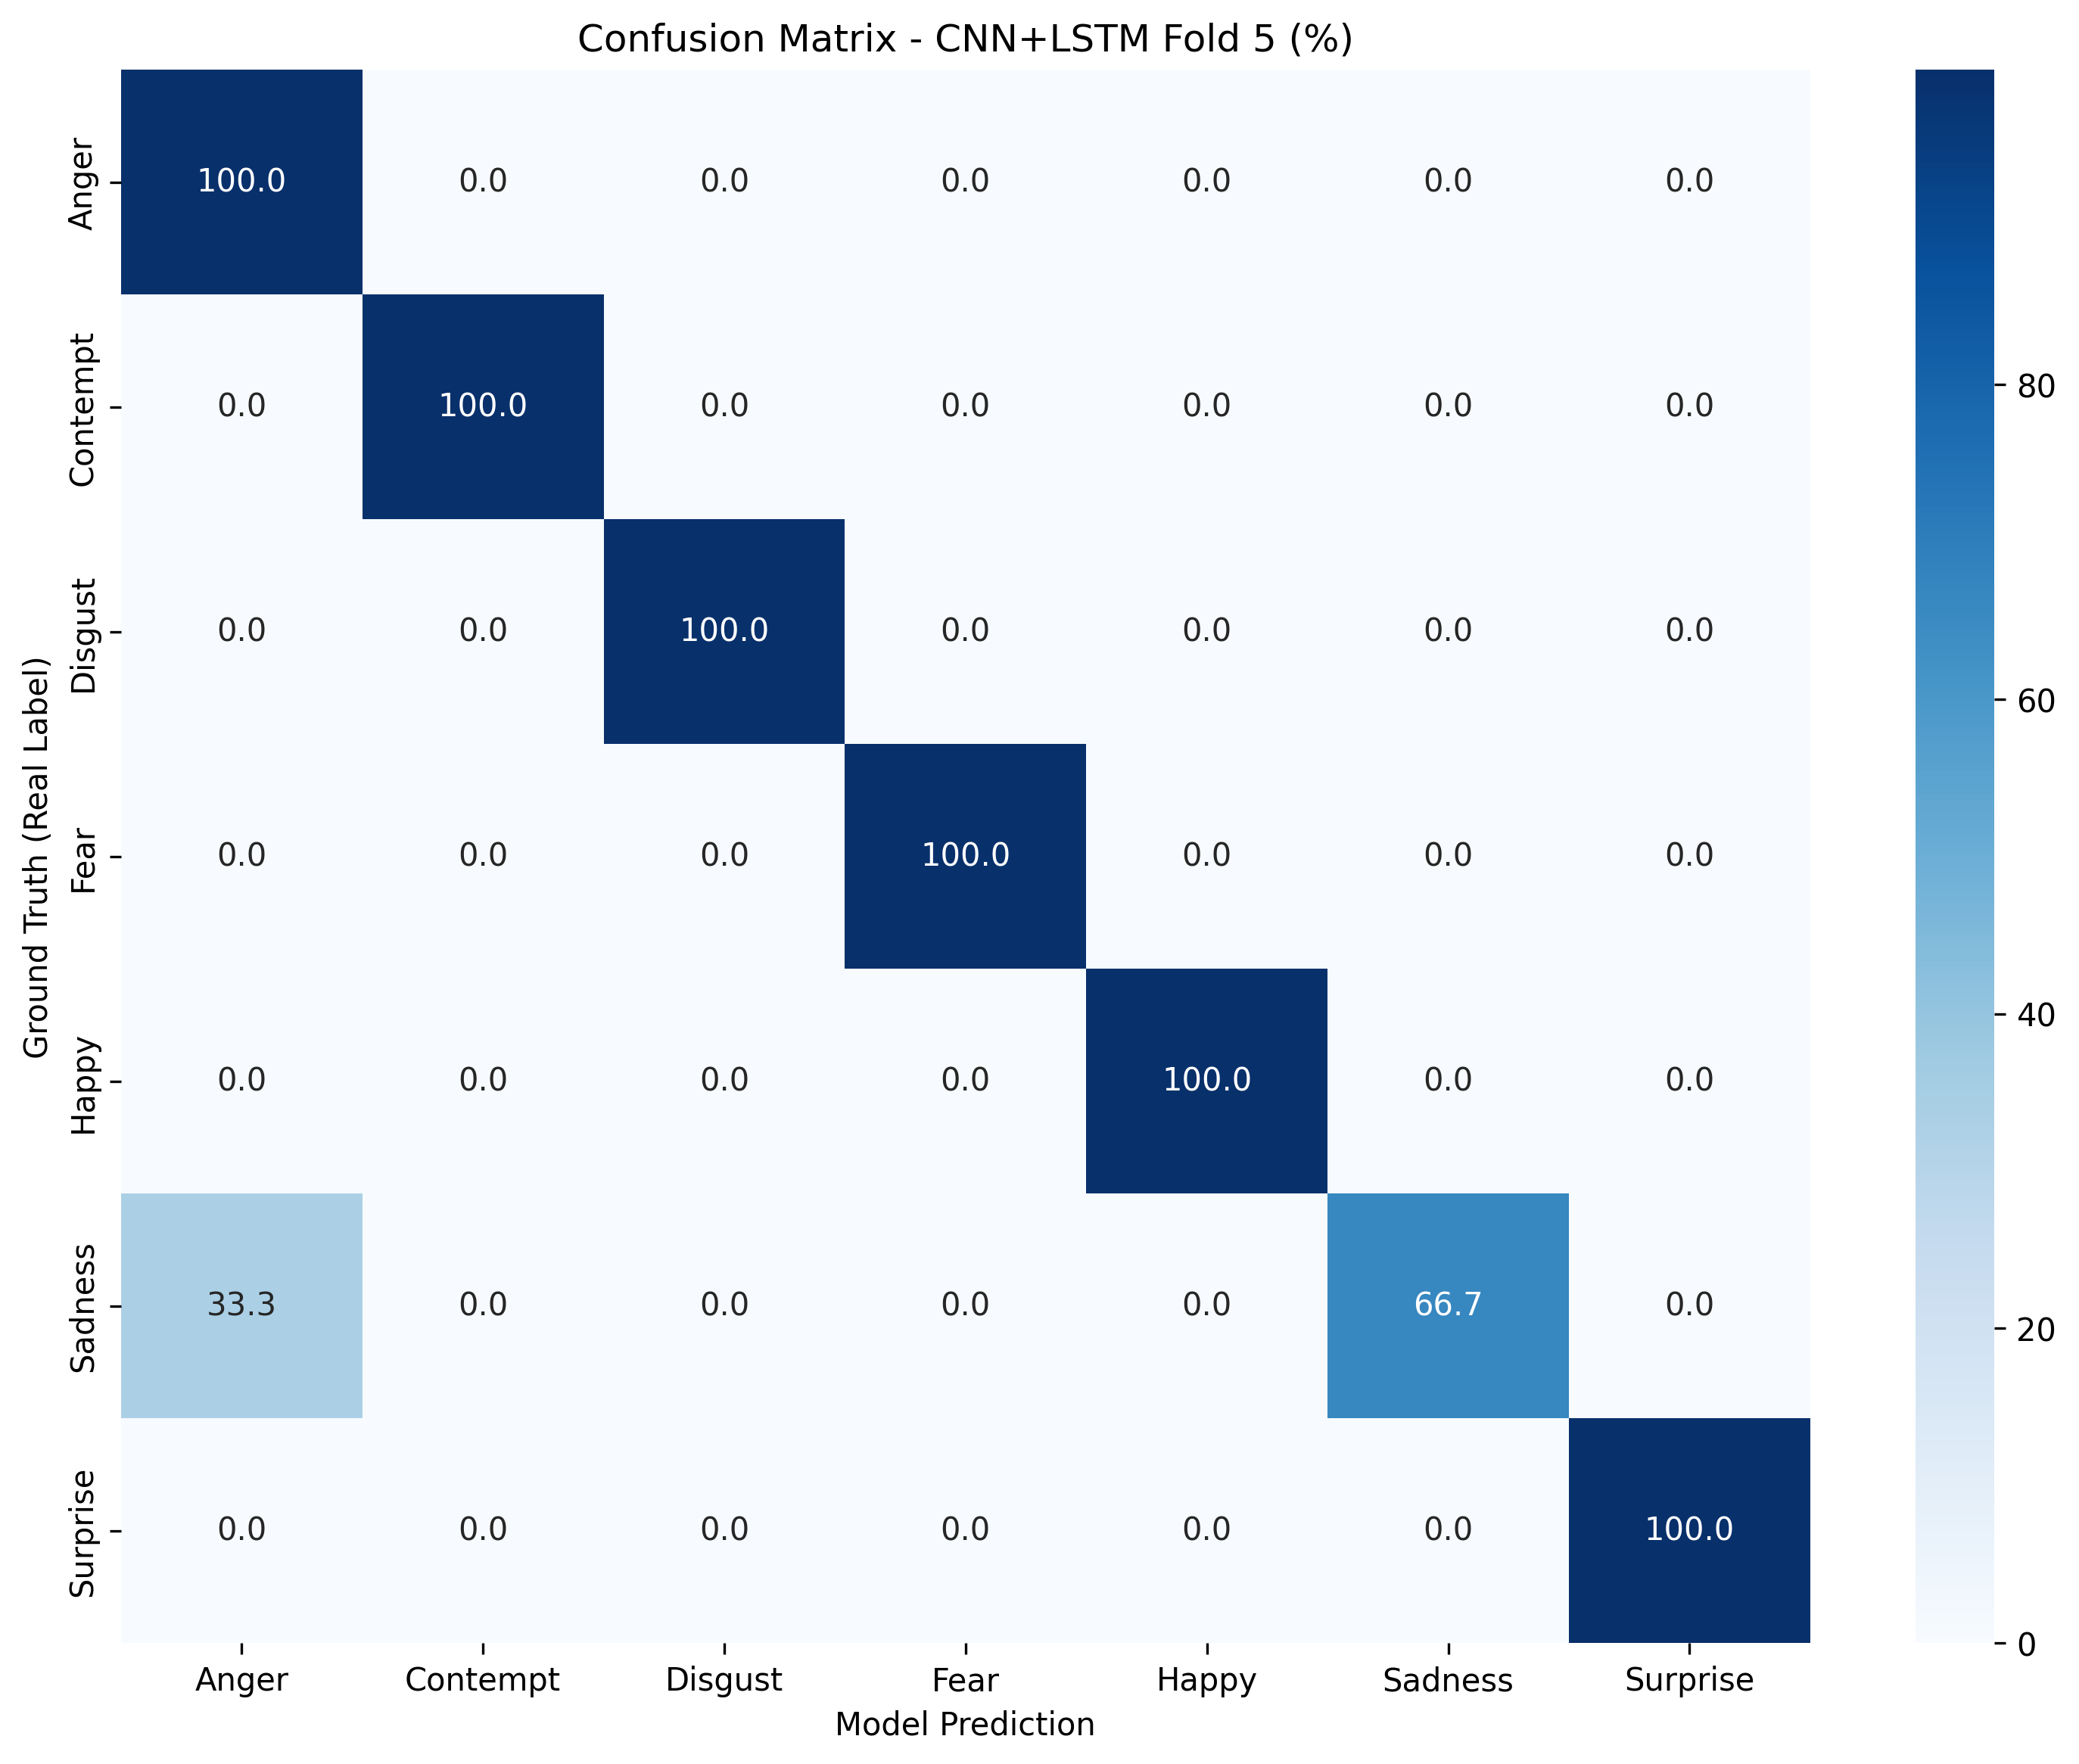
\includegraphics[width=0.7\textwidth]{figures/models/confusion_matrix_fold_5.png}
	\caption{Matricea de confuzie pentru CNN-LSTM (Fold 5). Se observă o singură eroare de clasificare.}
	\label{fig:cm_fold5}
\end{figure}

Singura eroare înregistrată a fost un eșantion din clasa \textbf{Sadness}, care a fost identificat eronat ca fiind \textbf{Anger}. Această confuzie este explicabilă prin tensiunea musculară similară în zona sprâncenelor (coborârea acestora) prezentă în ambele expresii în stadiul de apex.

\subsection*{Interpretarea deciziilor prin Grad-CAM}

Pentru a valida calitativ modelul, s-a utilizat tehnica \textbf{Grad-CAM (Gradient-weighted Class Activation Mapping)}. Aceasta permite vizualizarea zonelor feței pe care rețeaua s-a focalizat pentru a stabili eticheta emoțională. În Figura \ref{fig:gradcam_grid} sunt prezentate hărțile de activare pentru eșantioanele din Fold 5.

\begin{figure}[h!]
	\centering
	\begin{subfigure}{0.24\textwidth}
		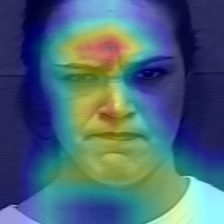
\includegraphics[width=\textwidth]{figures/models/gradcam_cnn+lstm_fold5/anger_pass.jpg}
		\caption{Anger}
	\end{subfigure}
	\begin{subfigure}{0.24\textwidth}
		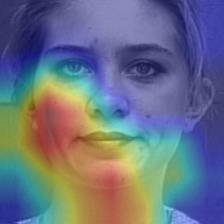
\includegraphics[width=\textwidth]{figures/models/gradcam_cnn+lstm_fold5/contempt_pass.jpg}
		\caption{Contempt}
	\end{subfigure}
	\begin{subfigure}{0.24\textwidth}
		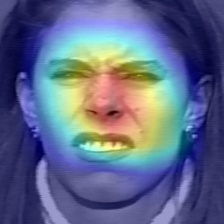
\includegraphics[width=\textwidth]{figures/models/gradcam_cnn+lstm_fold5/disgust_pass.jpg}
		\caption{Disgust}
	\end{subfigure}
	\begin{subfigure}{0.24\textwidth}
		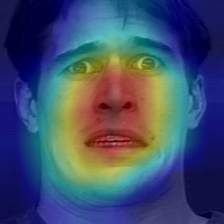
\includegraphics[width=\textwidth]{figures/models/gradcam_cnn+lstm_fold5/fear_pass.jpg}
		\caption{Fear}
	\end{subfigure}
	
	\vspace{0.2cm}
	
	\begin{subfigure}{0.24\textwidth}
		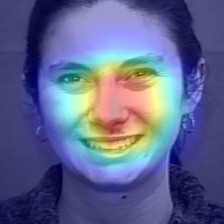
\includegraphics[width=\textwidth]{figures/models/gradcam_cnn+lstm_fold5/happy_pass.jpg}
		\caption{Happy}
	\end{subfigure}
	\begin{subfigure}{0.24\textwidth}
		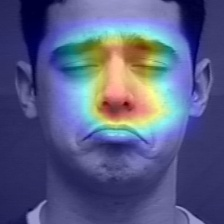
\includegraphics[width=\textwidth]{figures/models/gradcam_cnn+lstm_fold5/sad_pass.jpg}
		\caption{Sad (Corect)}
	\end{subfigure}
	\begin{subfigure}{0.24\textwidth}
		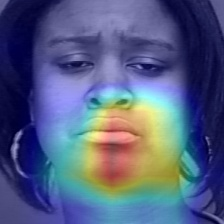
\includegraphics[width=\textwidth]{figures/models/gradcam_cnn+lstm_fold5/sad_FAIL_as_Anger.jpg}
		\caption{Sad $\to$ Anger}
	\end{subfigure}
	\begin{subfigure}{0.24\textwidth}
		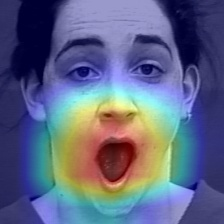
\includegraphics[width=\textwidth]{figures/models/gradcam_cnn+lstm_fold5/surprise_pass.jpg}
		\caption{Surprise}
	\end{subfigure}
	\caption{Vizualizarea regiunilor de interes prin Grad-CAM (Fold 5).}
	\label{fig:gradcam_grid}
\end{figure}

\subsubsection{Observații privind regiunile de interes}

Analiza hărților de activare a scos în evidență câteva aspecte contra-intuitive și interesante:

\begin{itemize}
	\item \textbf{Recunoașterea Fericirii (Happy):} Contrar așteptărilor, modelul nu se concentrează exclusiv pe zona gurii (zâmbet). Grad-CAM indică o activare intensă în \textbf{zona nasului} și a pliurilor nazolabiale. Acest lucru sugerează că modelul a învățat că lărgirea bazei nasului și ridicarea obrajilor sunt indicatori mai robuști pentru această clasă decât simpla deschidere a gurii.
	\item \textbf{Eroarea Sad vs. Anger:} În cazul eșantionului clasificat greșit, se observă că activarea Grad-CAM este localizată puternic între sprâncene. Modelul a interpretat contracția mușchiului \textit{corrugator supercilii} ca fiind specifică furiei, ignorând indiciile mai subtile de tristețe din jurul ochilor.
	\item \textbf{Surpriza:} Modelul prezintă o focalizare clară pe zona ochilor și a frunții, detectând ridicarea sprâncenelor, trăsătură anatomică definitorie pentru această emoție.
\end{itemize}

\section{Modelul ANN Echivalent: Izolarea Impactului Paradigmei de Spiking}

Pentru a determina în ce măsură performanța modelului bio-inspirat este influențată de arhitectura sa convoluțională versus mecanismul de spiking, a fost implementat un model \textbf{ANN Echivalent (Equivalent Baseline ANN)}. 

\subsection*{Arhitectură și Metodologie}
Acest model păstrează topologia hărților de trăsături ale CSNN-ului, dar înlocuiește neuronii de tip \textit{Leaky Integrate-and-Fire} cu unități de activare standard și învățare prin \textit{backpropagation}.

\begin{itemize}[noitemsep]
	\item \textbf{Configurație:} Strat convoluțional 3D (64 filtre, kernel $3 \times 5 \times 5$), urmat de \textit{Batch Normalization} și activare ReLU.
	\item \textbf{Pooling:} \texttt{AvgPool3d} ($2 \times 4 \times 4$), similar mecanismului de pooling din SNN.
	\item \textbf{Antrenare:} S-a utilizat optimizatorul Adam și funcția de cost \textit{Cross-Entropy}, fără augmentare de date, pentru a menține condițiile experimentale ale CSNN-ului.
	\item \textbf{Date de intrare:} S-au utilizat fețe pre-procesate (\textit{cropped}), eliminând fundalul pentru a permite modelului să conveargă rapid în absența augmentărilor.
\end{itemize}

\subsection*{Rezultate Experimentale}
Rezultatele pe cele 10 fold-uri sunt prezentate în Tabelul \ref{tab:rezultate_ann_echivalent}. Media obținută este de \textbf{73.23\%}, o valoare semnificativ superioară baseline-ului SVM, dar inferioară modelului complex CNN-LSTM.

\begin{table}[h!]
	\centering
	\caption{Performanța modelului ANN echivalent (3D Conv + ReLU)}
	\label{tab:rezultate_ann_echivalent}
	\begin{tabular}{lc|lc}
		\toprule
		\textbf{Fold} & \textbf{Acuratețe (\%)} & \textbf{Fold} & \textbf{Acuratețe (\%)} \\ \midrule
		Fold 1 & 75.76\% & Fold 6 & 67.86\% \\
		Fold 2 & 80.00\% & Fold 7 & 71.88\% \\
		Fold 3 & 72.73\% & Fold 8 & 65.52\% \\
		Fold 4 & 84.38\% & Fold 9 & 71.43\% \\
		Fold 5 & 69.70\% & Fold 10 & 73.08\% \\ \midrule
		\textbf{Medie} & \multicolumn{3}{c}{\textbf{73.23\%}} \\ \bottomrule
	\end{tabular}
\end{table}

\subsection*{Analiză Comparativă Finală}

Prezența acestui model în studiu permite o interpretare critică a rezultatelor:

\begin{enumerate}
	\item \textbf{Importanța Focalizării (Cropping):} Experimentele preliminare au arătat că utilizarea imaginilor complete (cu fundal) scade performanța ANN-ului la aproximativ 30-40\%. Acest lucru subliniază un avantaj teoretic al CSNN-ului: prin filtrarea On/Off și Latency Coding, SNN-ul este inherent mai robust la zgomotul de fundal (pixelii statici nu generează spike-uri), în timp ce un ANN clasic are nevoie de decuparea feței sau de volume masive de date pentru a ignora fundalul.
	\item \textbf{STDP vs. Backpropagation:} Diferența de la 48.02\% (SNN) la 73.23\% (ANN) reprezintă „costul” utilizării unei reguli de învățare locale și nesupervizate (STDP). Deși Backpropagation este mai precis, STDP oferă un avantaj major în termeni de eficiență energetică pe hardware neuromorfic și plauzibilitate biologică.
	\item \textbf{Concluzie:} Modelul ANN echivalent demonstrează că topologia 3D Conv este extrem de potrivită pentru setul CK+, dar eficiența implementării spike-based depinde critic de rafinarea mecanismelor de homeostazie și a pragurilor de activare.
\end{enumerate}